\documentclass[12pt]{article}
\usepackage{graphicx}
\usepackage{caption}
\usepackage{subcaption}
\usepackage{amsmath}
\usepackage{blindtext}
\usepackage{pdfpages}
\usepackage{xcolor}
\usepackage{authblk}
\usepackage{float}
\usepackage{kpfonts} 
\usepackage{titlesec} 
\usepackage{titling}
\usepackage{rotating} 
\usepackage{geometry}
\usepackage{hyperref}

% declaring hyperlink appearance
\hypersetup{
    colorlinks=true,
    linkcolor=blue, 
    citecolor=blue, 
    urlcolor=blue 
}

% Title formatting
\titleformat{\section}[block]{\huge\bfseries\centering}{}{0em}{}
\title{Detection and Classification of Defects on Printed Circuit Boards with Machine Learning\\\phantom{.}}

\date{\today}

% Definition of \maketitle
\makeatletter
\def\@maketitle{
\raggedright
\vspace*{-30mm}
\hspace*{-20mm}

\includegraphics[width=40mm]{./graphics/data_scientest_logo.png}\\[3ex]
\begin{center}
{\huge \bfseries \@title}\\[3ex]
{\large Faiza Waheed}\\[0.5ex]
{\large \href{mailto:w.faiza@gmx.de}{\textit{\textcolor{blue}{w.faiza@gmx.de}}}}\\
{\large \href{https://github.com/wfaiza}{\textit{\textcolor{blue}{https://github.com/wfaiza}}}}\\[3ex]
{\large Niels Hartano}\\[0.5ex]
{\large \href{mailto:niels@gmx.de}{\textit{\textcolor{blue}{nylz-ds@proton.me}}}}\\
{\large \href{https://github.com/taubenus}{\textit{\textcolor{blue}{https://github.com/taubenus}}}}\\[3ex]
{\large Gernot Gellwitz}\\[0.5ex]
{\large \href{mailto:gernot@gmx.de}{\textit{\textcolor{blue}{g-not@gmx.de}}}}\\
{\large \href{https://github.com/Kathartikon}{\textit{\textcolor{blue}{https://github.com/Kathartikon}}}}\\[3ex]
{\large Supervisor: Alban Thuet}\\[0.5ex]
{\large \href{mailto:alban@datascientest.com}{\textit{\textcolor{blue}{alban@datascientest.com}}}}\\
{\large \href{https://github.com/lokilone}{\textit{\textcolor{blue}{https://github.com/lokilone}}}}\\[3ex]
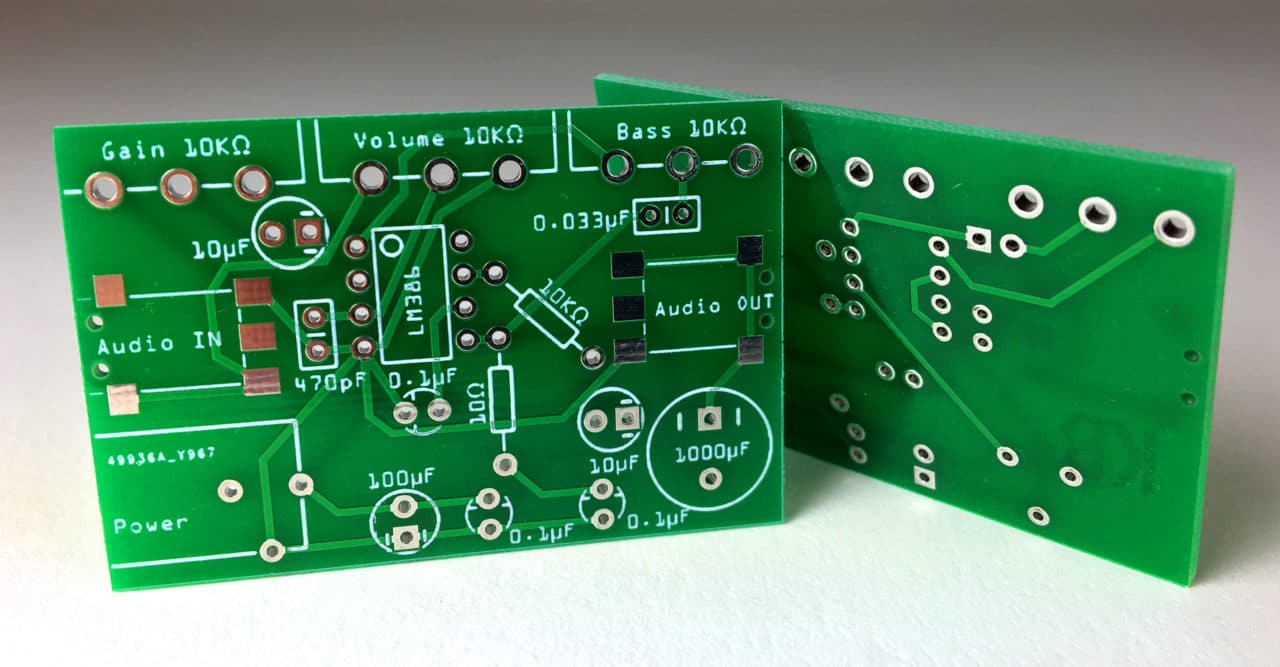
\includegraphics[width=110mm]{./graphics/PCB-Final-Image.jpg}\\[2ex]
{\large \href{https://github.com/wfaiza/PCB\_Defects\_Detection}{\textit{\textcolor{blue}{https://github.com/wfaiza/PCB\_Defects\_Detection}}}}\\[2ex]
\@date\\[2ex]
\end{center}}
\makeatother

\begin{document}

\thispagestyle{empty}
\maketitle
\thispagestyle{empty}

\tableofcontents
\thispagestyle{empty}
%Left indentation: \the\leftskip
%Right indentation: \the\rightskip
%\setlength{\leftskip}{-1em} 
%\setlength{\rightskip}{-1em} 

\clearpage
\newpage

\vspace{2.5cm}

\begin{abstract}

This report presents a machine learning approach for detecting and classifying defects on printed circuit boards (PCBs). The aim is to enhance the quality control process in PCB manufacturing by leveraging advanced computer vision techniques in observing and identifying various defects.  
\end{abstract}

\clearpage
\newpage

\section{Introduction}

Printed Circuit Boards (PCB's) are essential components in nearly all electronic devices. Ensuring their quality is critical, as defects can lead to device malfunctions or failures. Visual inspection, defect detection and recall are some of the most complex and expensive tasks for PCB manufacturing companies. Over the years, Printed Circuit Boards have become much smaller and more densely packed with components making the scalability of visual inspection harder. Traditional inspection methods, often manual, are time-consuming and prone to human error.

\begin{figure}[h]
    \centering
    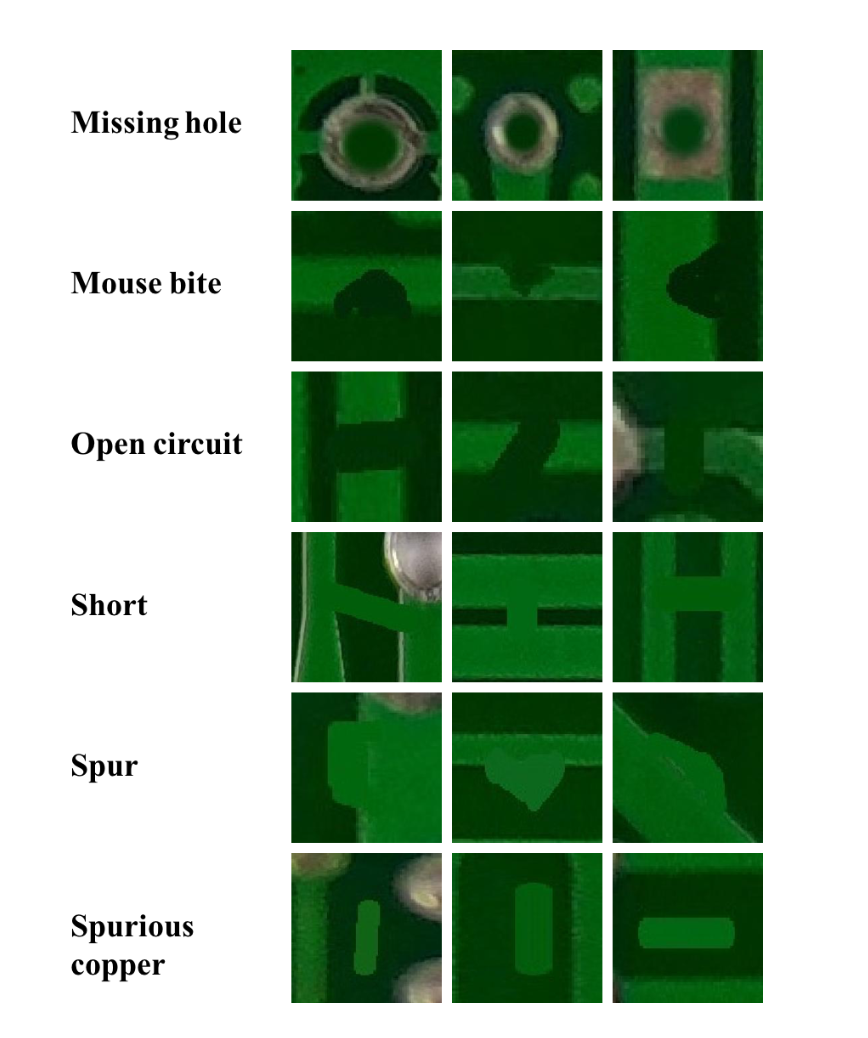
\includegraphics[width=0.6\textwidth]{./graphics/Defects.png}
    \caption{Sample defects explored in this project}
    \label{fig:defects}
\end{figure}

Machine learning, particularly deep learning, has shown significant promise in automating and improving the accuracy of defect detection and classification in PCB's. By training models on annotated images of PCB's, these systems can learn to identify various types of defects such as solder joint issues, component misalignment, and surface contamination (See Fig.~\ref{fig:defects}.). This quality assurance procedure ensures that the product quality is validated before it is marketed.

This project focuses on three approaches for defect detection and classification: the first approach is based on the VGG16 network, the second is based on a manually designed Convolution Neural Network U-Net model (including a residual connection block). While the third is based on YOLOv5 implementation. 
VGG16 makes use of so-called bounding boxes to detect defects, while the U-Net model uses mask segmentation (images) for detection and labels (label-encoded) for classification of defects. YOLOv5 also takes as input the encoded labels and bounding boxes coordinates for detection (segmentation and classification).

VGG16 can be downloaded as a pre-trained model from the TensorFlow Keras library, enabling transfer learning. In contrast, we developed and implemented the U-Net model from scratch. Similarly, YOLOv5 is available for download from Ultralytics. Leveraging these pre-trained models (VGG16 and YOLOv5), which have been trained on extensive datasets, allows us to harness their pretrained weights for training on our dataset, resulting in tangible improvements and robust performance.

A public PCB dataset containing over 10,000 images with 6 kinds of defects (Missing hole; Mouse bite; Open circuit; Short circuit; Spurious copper; Spur) was used for detection, classification and reporting tasks. This dataset is provided for public use and hosted on Kaggle.com, which is a community for data scientists and ML developers. The dataset is located at:\\ {\href{https://www.kaggle.com/datasets/akhatova/pcb-defects}{\textit{\textcolor{blue}{https://www.kaggle.com/datasets/akhatova/pcb-defects}}}}.

The dataset hosted on Kaggle is effectively sourced from the Open Lab on Human Robot Interaction of Peking University from\\
\href{https://robotics.pkusz.edu.cn/resources/datasetENG/}{\textit{\textcolor{blue}{https://robotics.pkusz.edu.cn/resources/datasetENG/}}}.\\
This is a large dataset of more than 10,000 PCB images with a total of around 22,000 annotated defects (classification and bounding box for defects), which we used to train and evaluate our models. The goal was to develop a robust system capable of detecting and classifying defects with high accuracy and efficiency.

\begin{figure}[h]
    \centering
    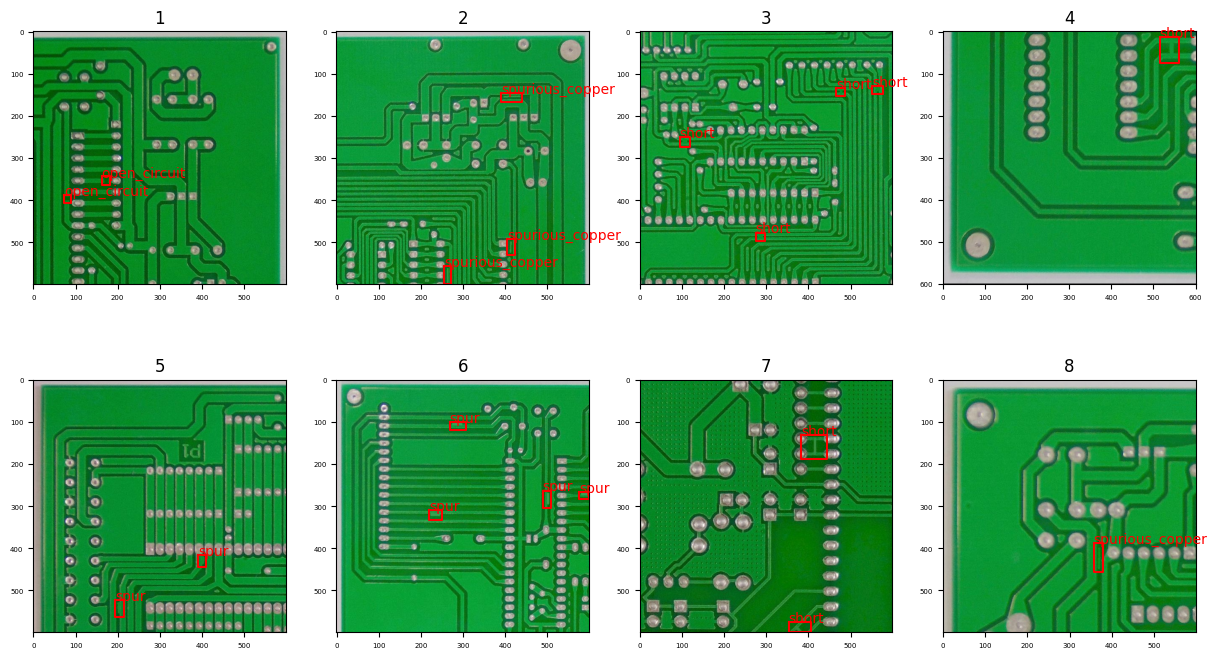
\includegraphics[width=1\textwidth]{./graphics/4.png}
    \caption{Sample images from the PCB dataset with annotated defects}
    \label{fig:sample_pcb_dataset}
\end{figure}

Some images only contained one defect, while others contained multiple defects (See Fig.~\ref{fig:sample_pcb_dataset}.), but the class of multiple defects for a single image was the same.

Over all, 6 different defects were considered for this project:
\begin{itemize}
    \item Mouse Bites
    \item Missing Holes
    \item Short circuit
    \item Spurious Copper
    \item Spur on trace
    \item Open Circuits
\end{itemize}
\begin{figure}[h]
    \centering
    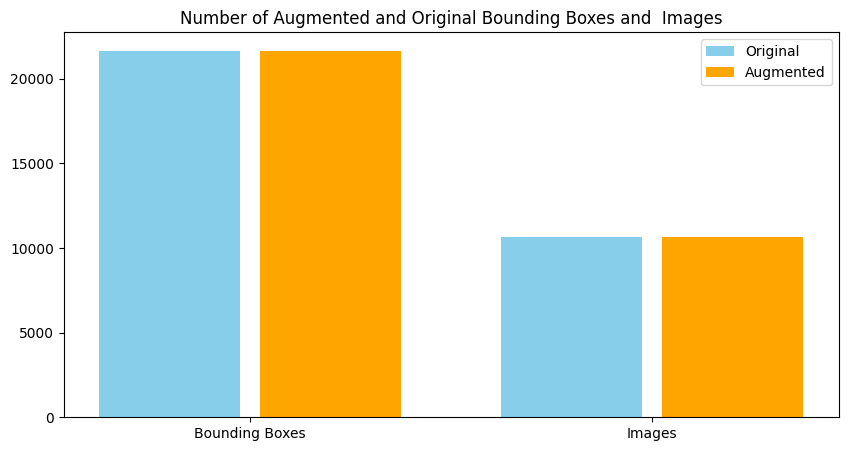
\includegraphics[width=0.8\textwidth]{./graphics/2.png}
    \caption{Ratio of Number of defects to Number of images for VGG16 model}
    \label{fig:ratio_dataset_vgg16}
\end{figure}

Initially the database seemed balanced, but that was from observing the class labeling for individual images. The defects appeared to be fairly distributed in the dataset, with the most common defect being "Mouse Bites" and the least common defect being "Shorts" (See Fig.~\ref{fig:defect_dist}.).

\begin{figure}[h]
    \centering
    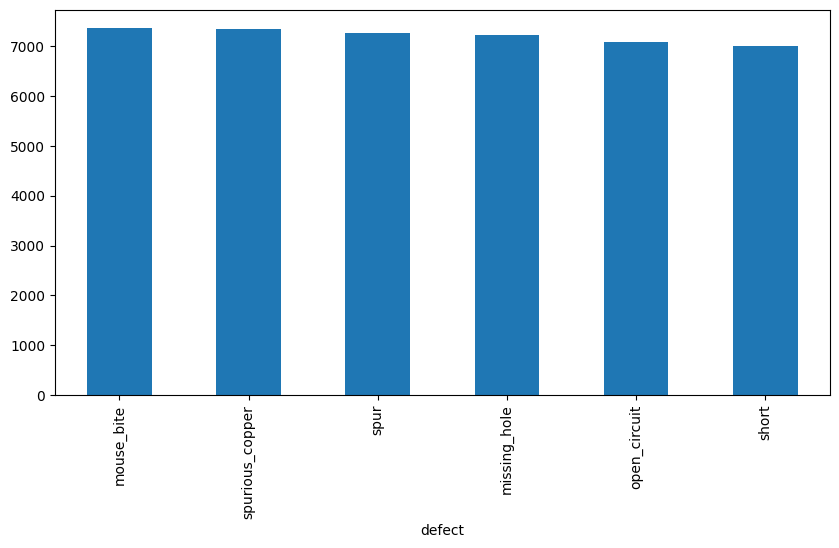
\includegraphics[width=0.8\textwidth]{./graphics/1.png}
    \caption{Defect distribution}
    \label{fig:defect_dist}
\end{figure}
The main objectives were to:
\begin{itemize}
    \item Create a data-frame from around 10.000 ".xml" annotation files in a ".csv" format containing the dimensions of the bounding boxes, size of the pictures and the class of defect.
    \item Pre-process the data which included resizing, sorting, ensuring that feature components were not distorted. 
    \item Populating the dataset by implementing image augmentations.
    \item Training machine learning model to detect and classify defects.
    \item Evaluate the model's performance and optimize it for potential deployment in a production environment.
\end{itemize}

\subsection{Pre-processing}
A high-quality dataset is crucial for training an effective model. Data augmentation is a crucial technique in machine learning, 
particularly for tasks involving image data, such as object detection and classification of defects on printed circuit boards (PCB's). 
By artificially expanding the training dataset through transformations like rotations, flips, scaling, and translations, data augmentation 
helps improve the robustness and generalization ability of the model. This process mitigates over-fitting by exposing the model to a diverse 
set of variations and scenarios that it might encounter in real-world applications. Consequently, data augmentation enhances the model's 
ability to accurately detect and classify defects, even when faced with new or slightly altered images, thereby improving its overall 
performance and reliability in practical deployment.
Two approaches were considered for data augmentation: Using a library or implementing the augmentations manually. The former is more convenient and less error-prone, while the latter offers more flexibility and control over the augmentation process. 

\subsubsection{Augmentations via Albumentations}

The library-based approach made use of the library "Albumentations", specifically techniques available like random brightness or contrast, random cropping of the image, rotation, horizontal or vertical flipping, including random sun flares or changing of the hue saturation value (See Fig.~\ref{fig:Albumentations}.).

\begin{figure}[h]
    \centering
    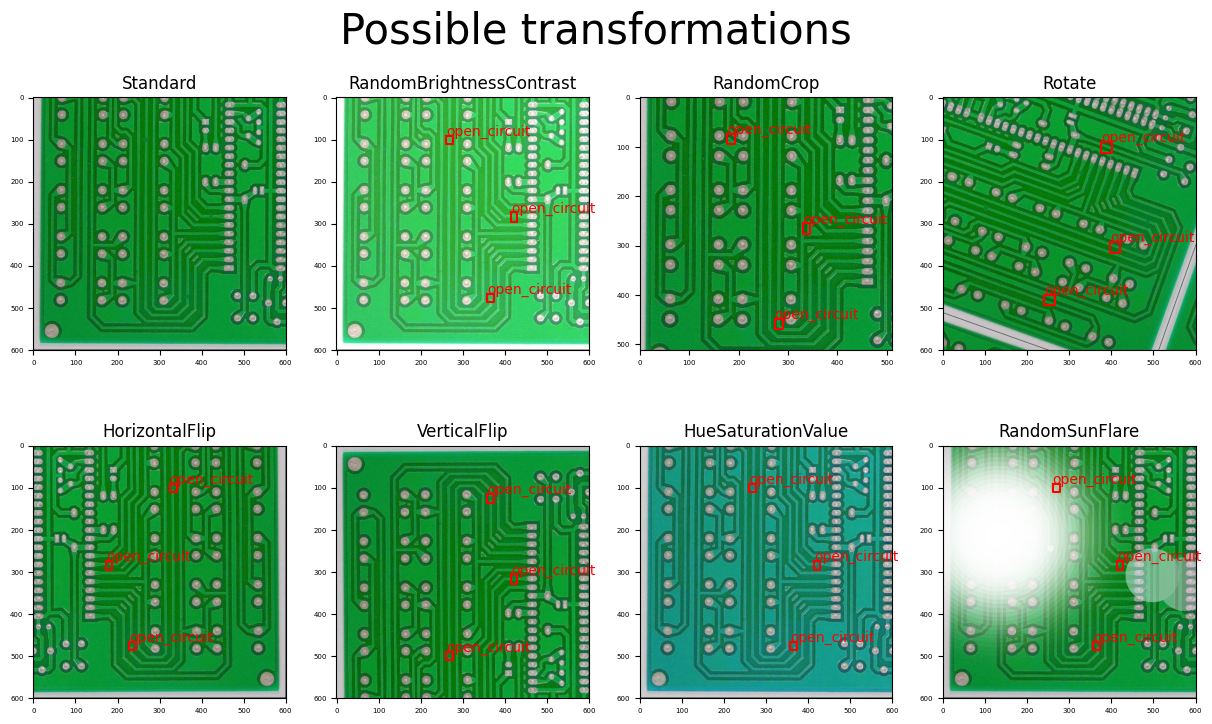
\includegraphics[width=0.8\textwidth]{./graphics/5.png}
    \caption{Possible augmentations by "Albumentations".}
    \label{fig:Albumentations}
\end{figure}

Problems that occurred during this process were that the cropping of the images may lead to the loss of the defect, if the defect is located outside of the cropped part of the image, which is not desired.
In this case the defect would not be detected by the model. Another problem was that in the case of rotation the defects were not correctly placed as can be seen in Fig.~\ref{fig:Albumentations}. This observation is why cropping and rotation were not used in the final VGG16 model.

\subsubsection{Manual Augmentations}
Let us now discuss the pre-processing that went into preparing the dataset before and after augmentation so that it would not lead to insufficient or inefficient training.

\begin{figure}[h]
    \centering
    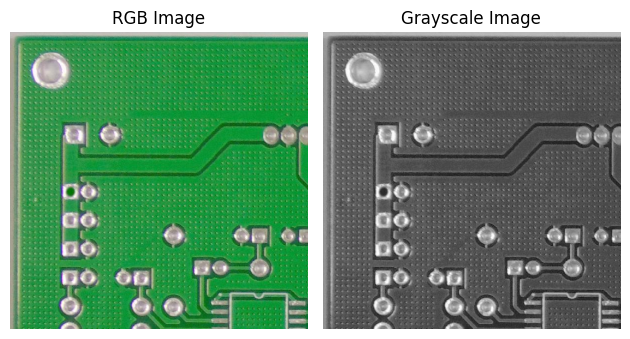
\includegraphics[width=0.8\textwidth]{./graphics/rgb vs grayscale.png}
    \caption{Colored vs. Grayscale image}
    \label{fig:Rgb_gray}
\end{figure}

Early on after observing the size of images (dim:600x600x3), we decided to crop the images to easily processable dimensions i.e. 100x100. Another decision was to convert the images to gray scale since that would improve computing power immensely while there would be no observable loss in the features of the images.

\begin{figure}[h]
    \centering
    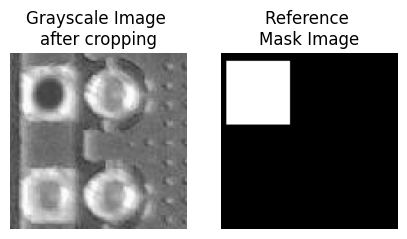
\includegraphics[width=0.8\textwidth]{./graphics/croppedimagewithmask.png}
    \caption{Cropping image and mask to 100x100 dimension}
    \label{fig:croppedimagewithmask}
\end{figure}

We observed various issues during the process of implementing on-the-fly augmentation by data generators like ImageDataGenerator on the dataset. We managed to solve some of those like instances where masks and labels were incorrectly referenced to the original image or adaption to our multi output structure (segmentation and classification) or insufficient control over the type of augmentation.  Others were harder to come by because they were intrinsic and needed solutions too complex to be practical. Similar to Albumentations; the  augmentation provided by DataImageGenerator performed rotation and zoom transformations differently on the images and their corresponding masks so that images and masks would not be aligned anymore after augmentation, or defects that were wholly or partially cropped by shift transformations. Considering all this we concluded that it would be beneficial to invest time in implementing manual augmentation for the cost of having to save all the augmented dataset to disk. For training a robust and reliable U-Net model, the following augmentation techniques were implemented (See Fig.~\ref{fig:manual_augmentation}.).:
\begin{figure}[h]
    \centering
    \begin{turn}{270}
    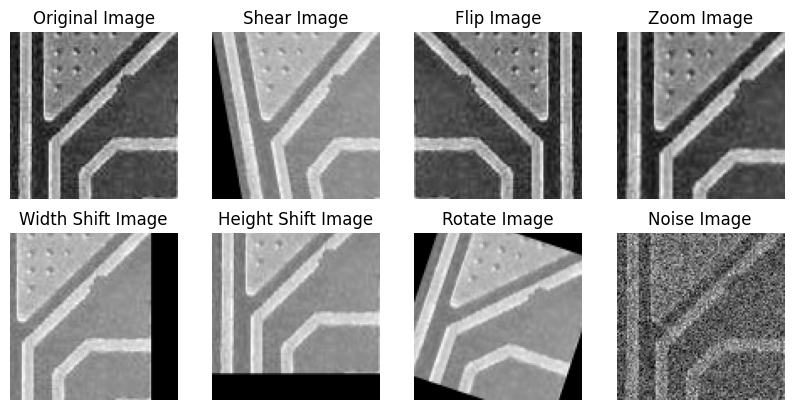
\includegraphics[width=1\textwidth]{./graphics/manual augmentation.png}
    \end{turn}
    \caption{Manually implemented augmentations}
    \label{fig:manual_augmentation}
\end{figure}

\begin{itemize}
    \item Rotation the image 
    \item Shifting the image horizontally  
    \item Shifting the image vertically  
    \item Shearing the image
    \item Enlarging or reducing  the image
    \item Horizontally flipping the image 
    \item Introducing Gaussian noise to the image
\end{itemize}

To implement cropping on the dataset, we had to keep in mind that the relevant label/defect class would be properly referenced. In our case, we had to introduce the "none" class to offset the generation of cropped images that had no "defects".

While preprocessing the dataset, we also observed that sometimes the defect would be located in the cropping boundary of the image. If we implemented the cropping without any intervention, the cropped image would not provide a good feature set for the model to train on. Hence we implemented a boundary shifting function which ensured that the defect would not be cropped.

Another observation was that while augmentation, if the defect was located at the boundary of the image, sometimes it would remove the defect from the image after implementing the augmentation
technique. Hence we had to implement a check to ensure that the relevant features were not lost. With these checks and balances, we managed to ensure that the dataset for training the model was balanced, relevant and not suffering from feature loss.
As already mentioned, the images in the dataset have single and multiple defects in a single instance (image). Therefore, we had to cater for the cases in which there were multiple defects in a single image so that the model could process the mask and label for the defects accordingly. We brainstormed on how to handle such instances and agreed on removing multiple defects from a single image and separating all defects into single image instances. For this we implemented a defect separation function.

\clearpage
\newpage

\section{Modelling}
The methodology of this project involves several key steps: data set generation and preprocessing, model design and training, and evaluation. As discussed above; the dataset generation and preprocessing was handled manually. Now we will discuss the design and training of the various image processing models.

\subsection{Model Design and Training}

\subsubsection{VGG16}

The VGG16 model is a Convolutional Neural Network architecture that has been widely used for image classification tasks. It consists of 16 layers, including 13 convolutional layers and 3 fully connected layers. The model has been pre-trained on the ImageNet dataset, which contains millions of images across thousands of classes. By leveraging transfer learning, we can take advantage of the features learned by the model on ImageNet and fine-tune it on our PCB dataset.
The model was implemented using the TensorFlow and Keras libraries. 

VGG16 requires the following additional preprocessing steps: 

\begin{itemize}
    \item Resizing images to a 224 by 224 image size to fit the model input requirements. All colors where kept
    \item Normalizing pixel values to the range [0, 1].  
\end{itemize}

Furthermore the dimensions of the bounding box where normalized and centered. The defects had to be split up by using a One Hot Encoding. The dataset was then split into a training and a validation set. 
TensorFlow additionally requires the transformation of the dataset into a tf.data.Dataset object.

Two approaches were tested: freezing (keeping) all pretrained layers and only adding a flatten layer and an detection and an classification head and unfreezing all layers.

\begin{figure}[h]
    \centering
    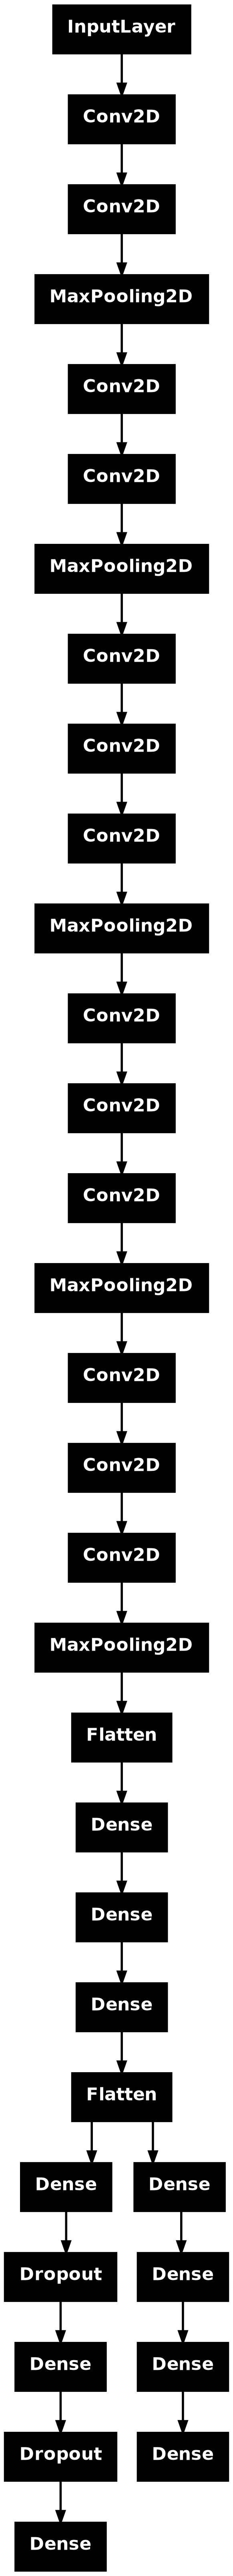
\includegraphics[width=0.14\textwidth]{./graphics/3.png}
    \caption{VGG16 with two pathways/modules.}
\end{figure}

By integrating separate pathways/modules, different loss functions and metrics can be applied to each task. Hence, our implementation enabled us to use different loss functions and metrics for the detection and classification task. 
For the detection task the loss function GIoU and metrics One-Hot-IOU was used, while for the classification task the loss function categorical cross-entropy and metrics accuracy were used.

To avoid unnecessary computation, callbacks were implemented such as early stopping and model checkpoint. 

Unfortunately, we are currently still trying to get this implementation to work. So hopefully in the future results will be shared once this model is successfully implemented. 

\clearpage
\newpage

\subsubsection{U-Net}
For the development and implementation of our machine learning model, we went through many design iterations to finally decide on the RES-UNET model scheme (See Fig.~\ref{fig:resunetmodel}.).

The RES-UNET model provides the combined qualities of a Residual network connection to enhance feature extraction at every stage of the Unet network architecture. With the help of having the Residual connection, the model has ease of learning by removing the vanishing gradient problem along with robust feature extraction. The U-net architecture ensures with the help of skip connection, that the high resolution features, which we need in our case for the defect segmentation task (object detection), are combined from the encoder and decoder to preserve spatial information.

As our task is to classify and detect the defects, we need both segmentation and classification outputs. This model handles both required outputs for a single instance simultaneously. We did entertain the idea of having separate models for obtain the two outputs, but decided to explore this combinatorial model architecture implementation instead.

Using two different branches/modules enables us to employ different loss functions (while emphasizing the loss weights for the training) and metrics for the detection and classification tasks.

We also utilized the various callbacks (timing, early-stopping, reduce-learning-rate and checkpoint) to avoid over-fitting and over-computation by unnecessary training. 

\newgeometry{left=-3cm, right=-3cm, top=-3cm, bottom=-3cm}
\begin{figure}[p]
    \centering
    \begin{turn}{270}
    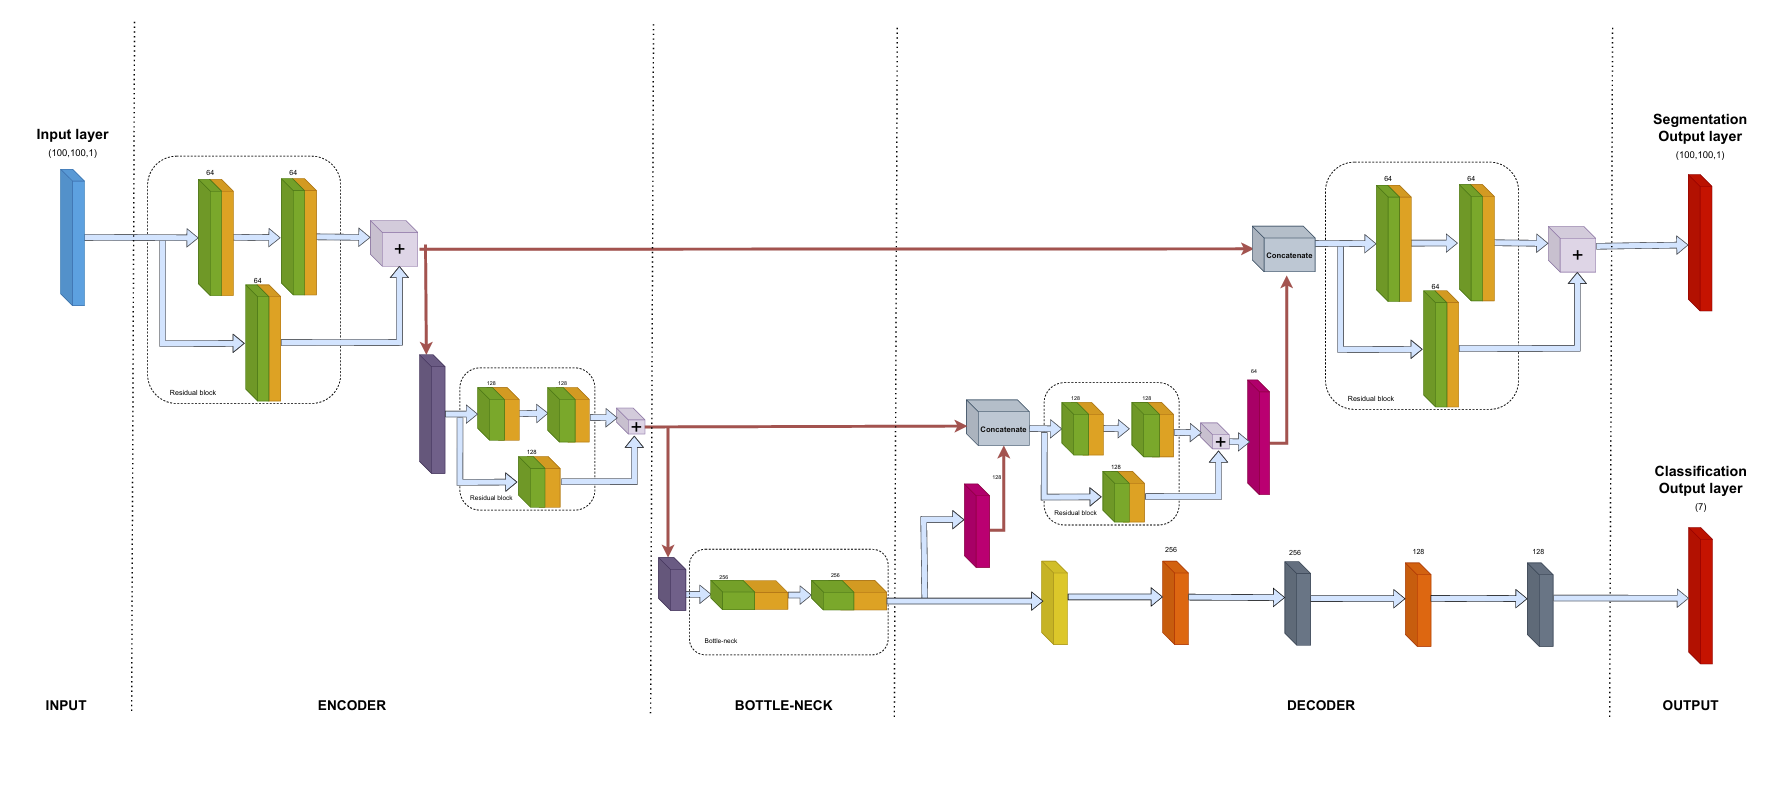
\includegraphics[width=1.2\paperwidth,height=1.2\paperheight,keepaspectratio]{./graphics/model-unet.png}
    \end{turn}
    \caption{RES-UNET model with 2 Modules/Outputs}
    \label{fig:resunetmodel}
\end{figure}
\restoregeometry

\clearpage
\newpage


\subsubsection{YOLOv5}
In addition to designing and developing our model for training, we also successfully implemented the YOLOv5 object detection model developed by Ultralytics on the PCB dataset. Unlike the original YOLO models built on DarkNet, YOLOv5 is developed with PyTorch, which enhances ease of understanding and usage.

This model can be utilized for both segmentation and classification, providing us with the opportunity to compare the results of our model with this pretrained and well-established design.

YOLOv5 uses input images in RGB format with a resolution of 640 pixels, which suits our dataset. Our image data has a resolution of 600 pixels. YOLOv5 provides the feature of passing images directly to the model for image augmentation automatically. During testing, it was observed that passing the images as-is (600 pixels) did not provide optimal results. Therefore, the images and corresponding labels were padded to resize them to 640 pixels to get the best results.

For reference, the YOLOv5 model architecture is elaborated in Fig.~\ref{fig:yolov5model}. For more details on model architecture please go to:\\

\href{https://docs.ultralytics.com/yolov5/tutorials/architecture_description}{\textit{\textcolor{blue}{https://docs.ultralytics.com/yolov5/tutorials/architecture\_description}}}

\newgeometry{left=-3cm, right=-3cm, top=-3cm, bottom=-3cm}
\begin{figure}[p]
    \centering
    \begin{turn}{270}
    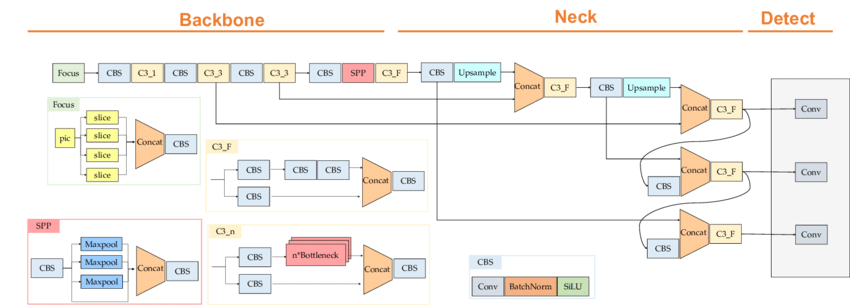
\includegraphics[width=1\paperwidth,height=1\paperheight,keepaspectratio]{./graphics/YOLOv5-architecture.png}
    \end{turn}
    \caption{YOLOv5 model architecture from \cite{Kim2021} available under CC BY 4.0.}
    \label{fig:yolov5model}
\end{figure}
\restoregeometry

After the required data augmentation, the model can start training with the following command:
!python path/to/train.py --data /path/to/data.yaml --weights yolov5s.pt --img 640 --epochs 50 --batch-size 16 --cache

In the current iteration of our training, we used the default Confidence and IoU thresholds (conf-thres=0.25 and iou-thres=0.45). The model was trained for 50 epoch, with batch size as 16. The pretrained small model (yolov5s.pt) weights were used. Potentially with further fine tuning training it can be done by freezing some layers and training on the desired layers. The choice to train on small model is because of the computational restrictions of our personal computers and also time restrictions. The results were compelling enough that it presents a good solution for our current object detection project. The output results for the models are discussed in the next section.

\clearpage
\newpage

\subsection{Evaluation}

The performance of the models was evaluated using accuracy, MeanIoU, precision, recall, and F1-score metrics. The VGG16 model unfortunately could not achieve any results but for the YOLOv5 model we achieved a classification accuracy of ~95\%, while with the U-Net model, we achieved a classification accuracy of ~90\%. 

Despite the high accuracy, both models faced challenges in detecting certain defects. The U-Net model struggled with detecting small defects, while the YOLOv5 model had difficulty distinguishing between similar defect types. The results are discussed in detail below.

\subsubsection{U-net}

The size of our validation set is 20\% of the cropped, separated, balanced and pre-augmented original training set. This means there are around 400 validation samples. The evaluation metrics are based on these samples. The defect ratios can be seen in Fig.~\ref{fig:val_set}.
\begin{figure}[H]
    \begin{center}
        \begin{tabular}{|c|c|}
            \hline
            Defect & Count\\
            \hline
            Missing Hole & 65 \\
            Mouse Bite & 55 \\
            Open Circuit & 59 \\
            Short & 57 \\
            Spur & 65 \\
            Spurious Copper & 47 \\
            None & 65\\
            \hline
        \end{tabular}
    \end{center}
    \caption{Validation Set Composition}
    \label{fig:val_set}
\end{figure}

The graphs in Fig.~\ref{fig:graphs_unet} show the development of different metrics during the final training epochs. We used Binary-Cross-Entropy and Categorical-Cross-Entropy as loss functions for the segmentation and classification outputs, respectively. The respective activation functions have been Sigmoid (binary) and Softmax (multi-class). Validation accuracy for segmentation is above 93\% already after the first training (20 epochs with loss weights 80/20 seg/class) and reaching 97\% after the final training (20 epochs with loss weights inverted i.e. 20/80 seg/class). It is not before the 10th epoch that the validation accuracy for classification is reaching 70\%. Same holds for classification precision and recall.


\begin{figure}[H]
    \centering
    %\begin{turn}{270}
    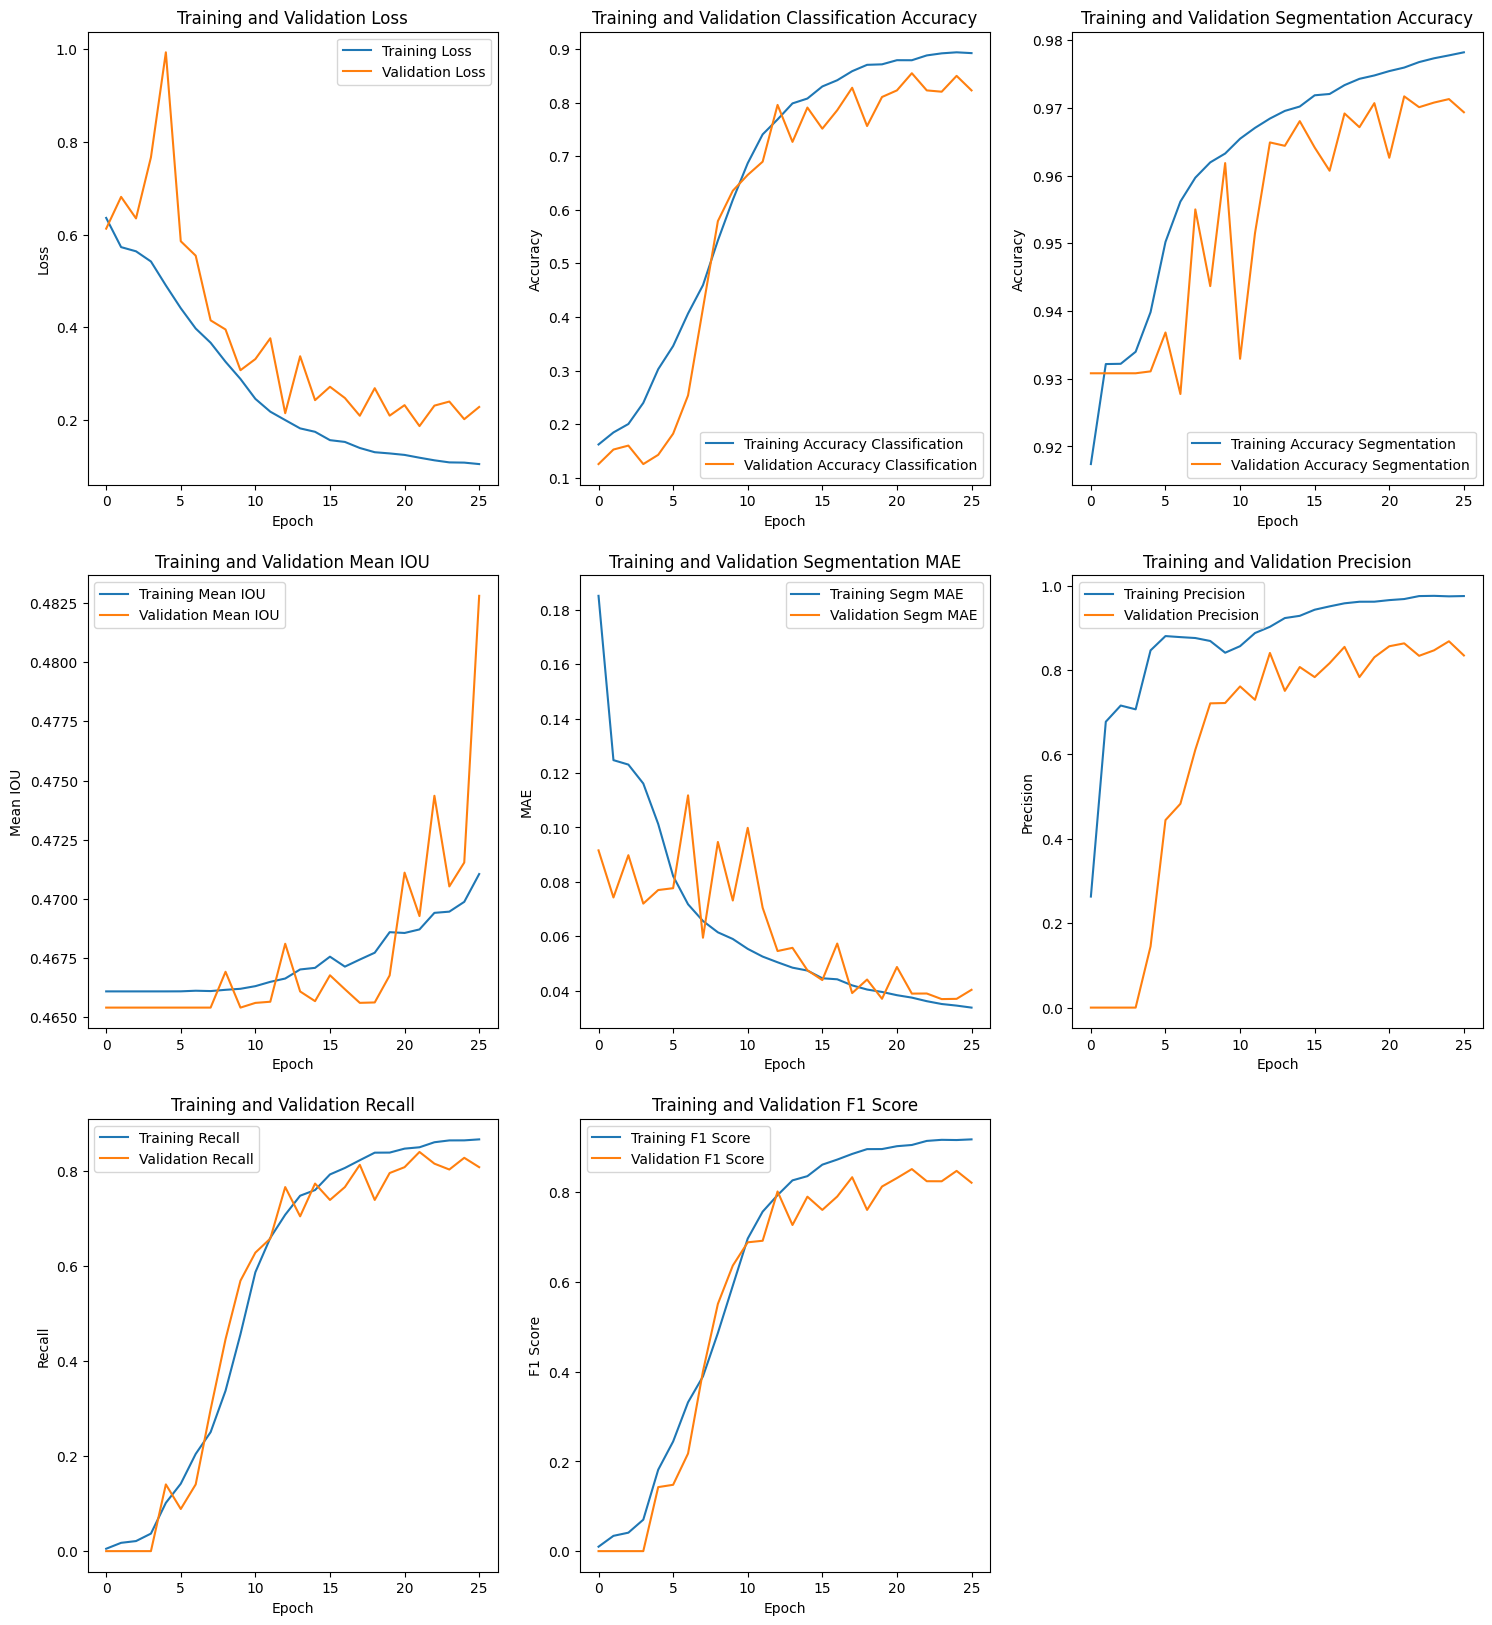
\includegraphics[width=\textwidth, keepaspectratio]{./graphics/graphs_vertical.png}
    %\end{turn}
    \caption{Metrics for Res-Unet model}
    \label{fig:graphs_unet}
\end{figure}
\restoregeometry
\clearpage


We can observe some encouraging results from the validation of the U-net model. The metrics' graphs show improvement still which indicates that the model will improve with training over more epochs. 
Graphs for U-net model : (See Fig.~\ref{fig:graphs_unet}.).

The confusion matrix (See Fig.~\ref{fig:confusion_unet}) and the classification report (See Fig.~\ref{fig:classification_report_unet}.) on the validation set show that precision and recall for each defect class vary but they are generally stable. 98\% of the short circuit detections on the test set are correct, while 24\% of the detected "spur" belong to a different class. Likewise, 98\% of the missing holes are correctly identified, while 20\% of the "none", "mouse-bite" and "spurious-copper" class are erroneously detected as "spur" or incorrectly detected. Hence we can observe that the defect classes of "spurious copper", "spur" and " mouse bites" are the most difficult to detect accurately. 

Confusion matrix : (See Fig.~\ref{fig:confusion_unet}.).
\newgeometry{left=-3cm, right=-3cm, top=-3cm, bottom=-3cm}
\begin{figure}[p]
    \centering
    \begin{turn}{270}  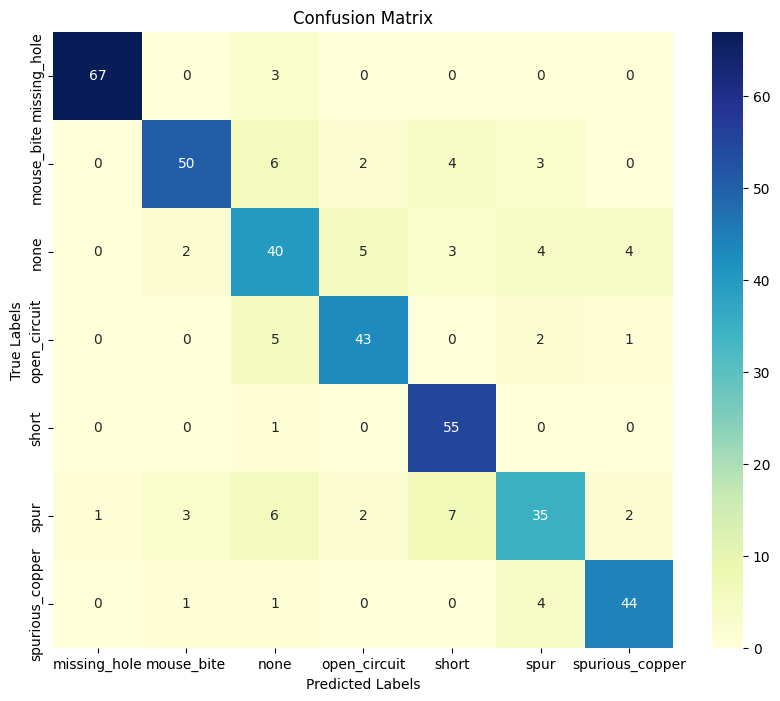
\includegraphics[width=0.7\paperwidth,height=0.7\paperheight,keepaspectratio]{./graphics/confusionmatrix_unet.png}
    \end{turn}
    \caption{Confusion Matrix for classification output}
    \label{fig:confusion_unet}
\end{figure}
\restoregeometry
\begin{figure}[H]
    \centering
    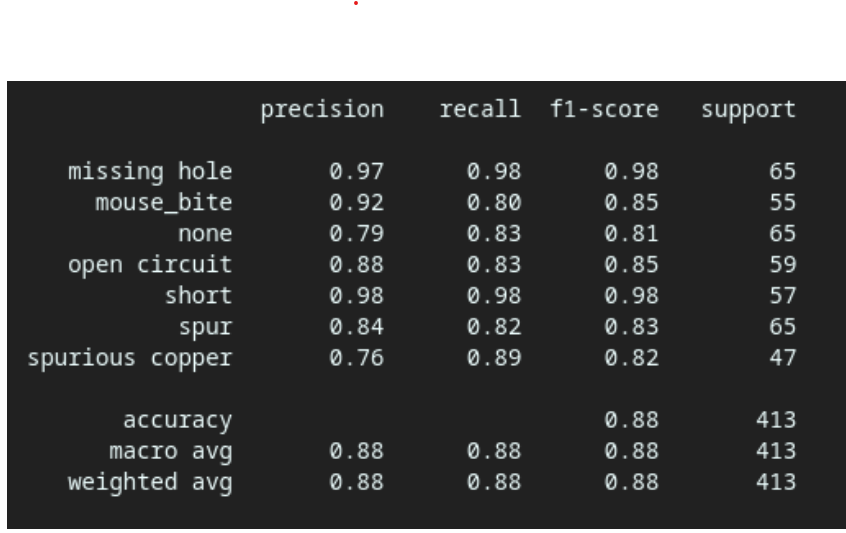
\includegraphics[width=0.7\textwidth]{./graphics/classification_report_unet.png}
    \caption{Classification metrics for classification output}
    \label{fig:classification_report_unet}
\end{figure}

\clearpage
%\newpage

\subsubsection{U-net model Results}
Fig.~\ref{fig:results1_unet} and Fig.~\ref{fig:results2_unet} illustrate that the location of the defects or the pixel matrix is predicted quite precisely. For clarification the real and predicted classes are shown.
															  
\begin{figure}[h]
    \centering
    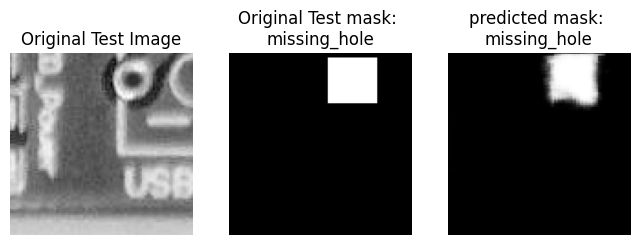
\includegraphics[width=0.8\textwidth]{./graphics/output1.png}
    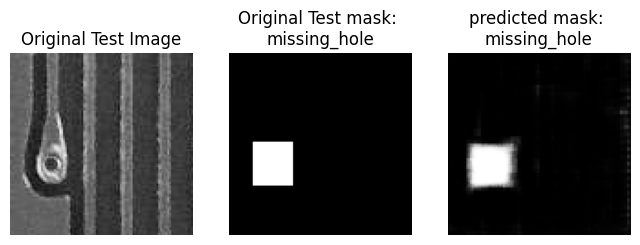
\includegraphics[width=0.8\textwidth]{./graphics/output2.png}
    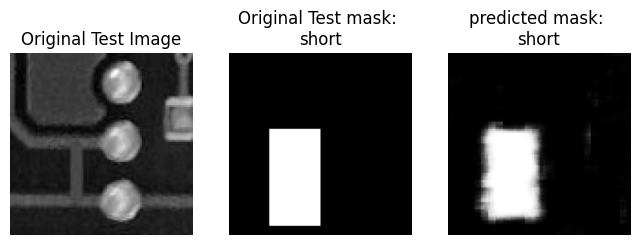
\includegraphics[width=0.8\textwidth]{./graphics/output3.png}

    \caption{Validation Results}
    \label{fig:results1_unet}
\end{figure}
\begin{figure}[h]
    \centering
    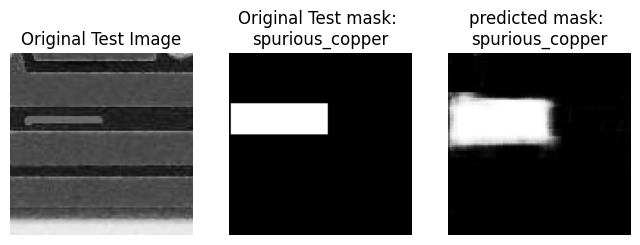
\includegraphics[width=0.8\textwidth]{./graphics/output4.png}
    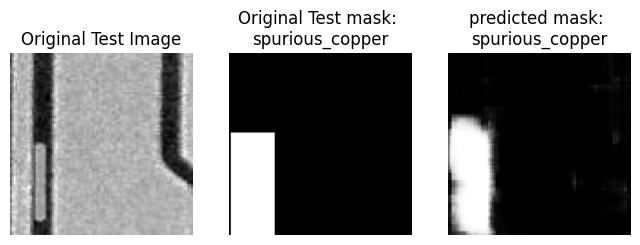
\includegraphics[width=0.8\textwidth]{./graphics/output5.png}
    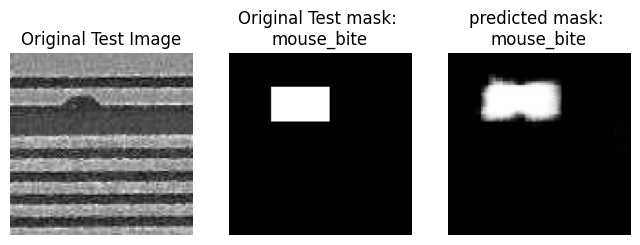
\includegraphics[width=0.8\textwidth]{./graphics/output6.png}
    \caption{Validation Results}
    \label{fig:results2_unet}
\end{figure}

\clearpage
\newpage

\subsubsection{YOLOv5}
The model was trained for 50 epochs and it can be observed from the resulting graphs that the training is still improving hence for further tests we can train the model over more epochs, though by observing the fluctuations in the validation loss, we can argue that model might be moving towards over fitting. The results are observably accurate already with just "Mouse-bite" and "Spur" type of defect giving issues to the model. The "Missing-hole" defect is the easiest for the model to detect, compounding the observation from the U-net model results which also performed the best for this type of defect.
The model was trained on pretrained weights for YOLOv5s since this is a small to medium size dataset. In future, training with fine tuning self-initialized weights can improve the results especially in case of over fitting.

Graphs for YOLOv5 model : (See Fig.~\ref{fig:graphs_yolo}.).
\newgeometry{left=-3cm, right=-3cm, top=-3cm, bottom=-3cm}
\begin{figure}[p]
    \centering
    \begin{turn}{270}
    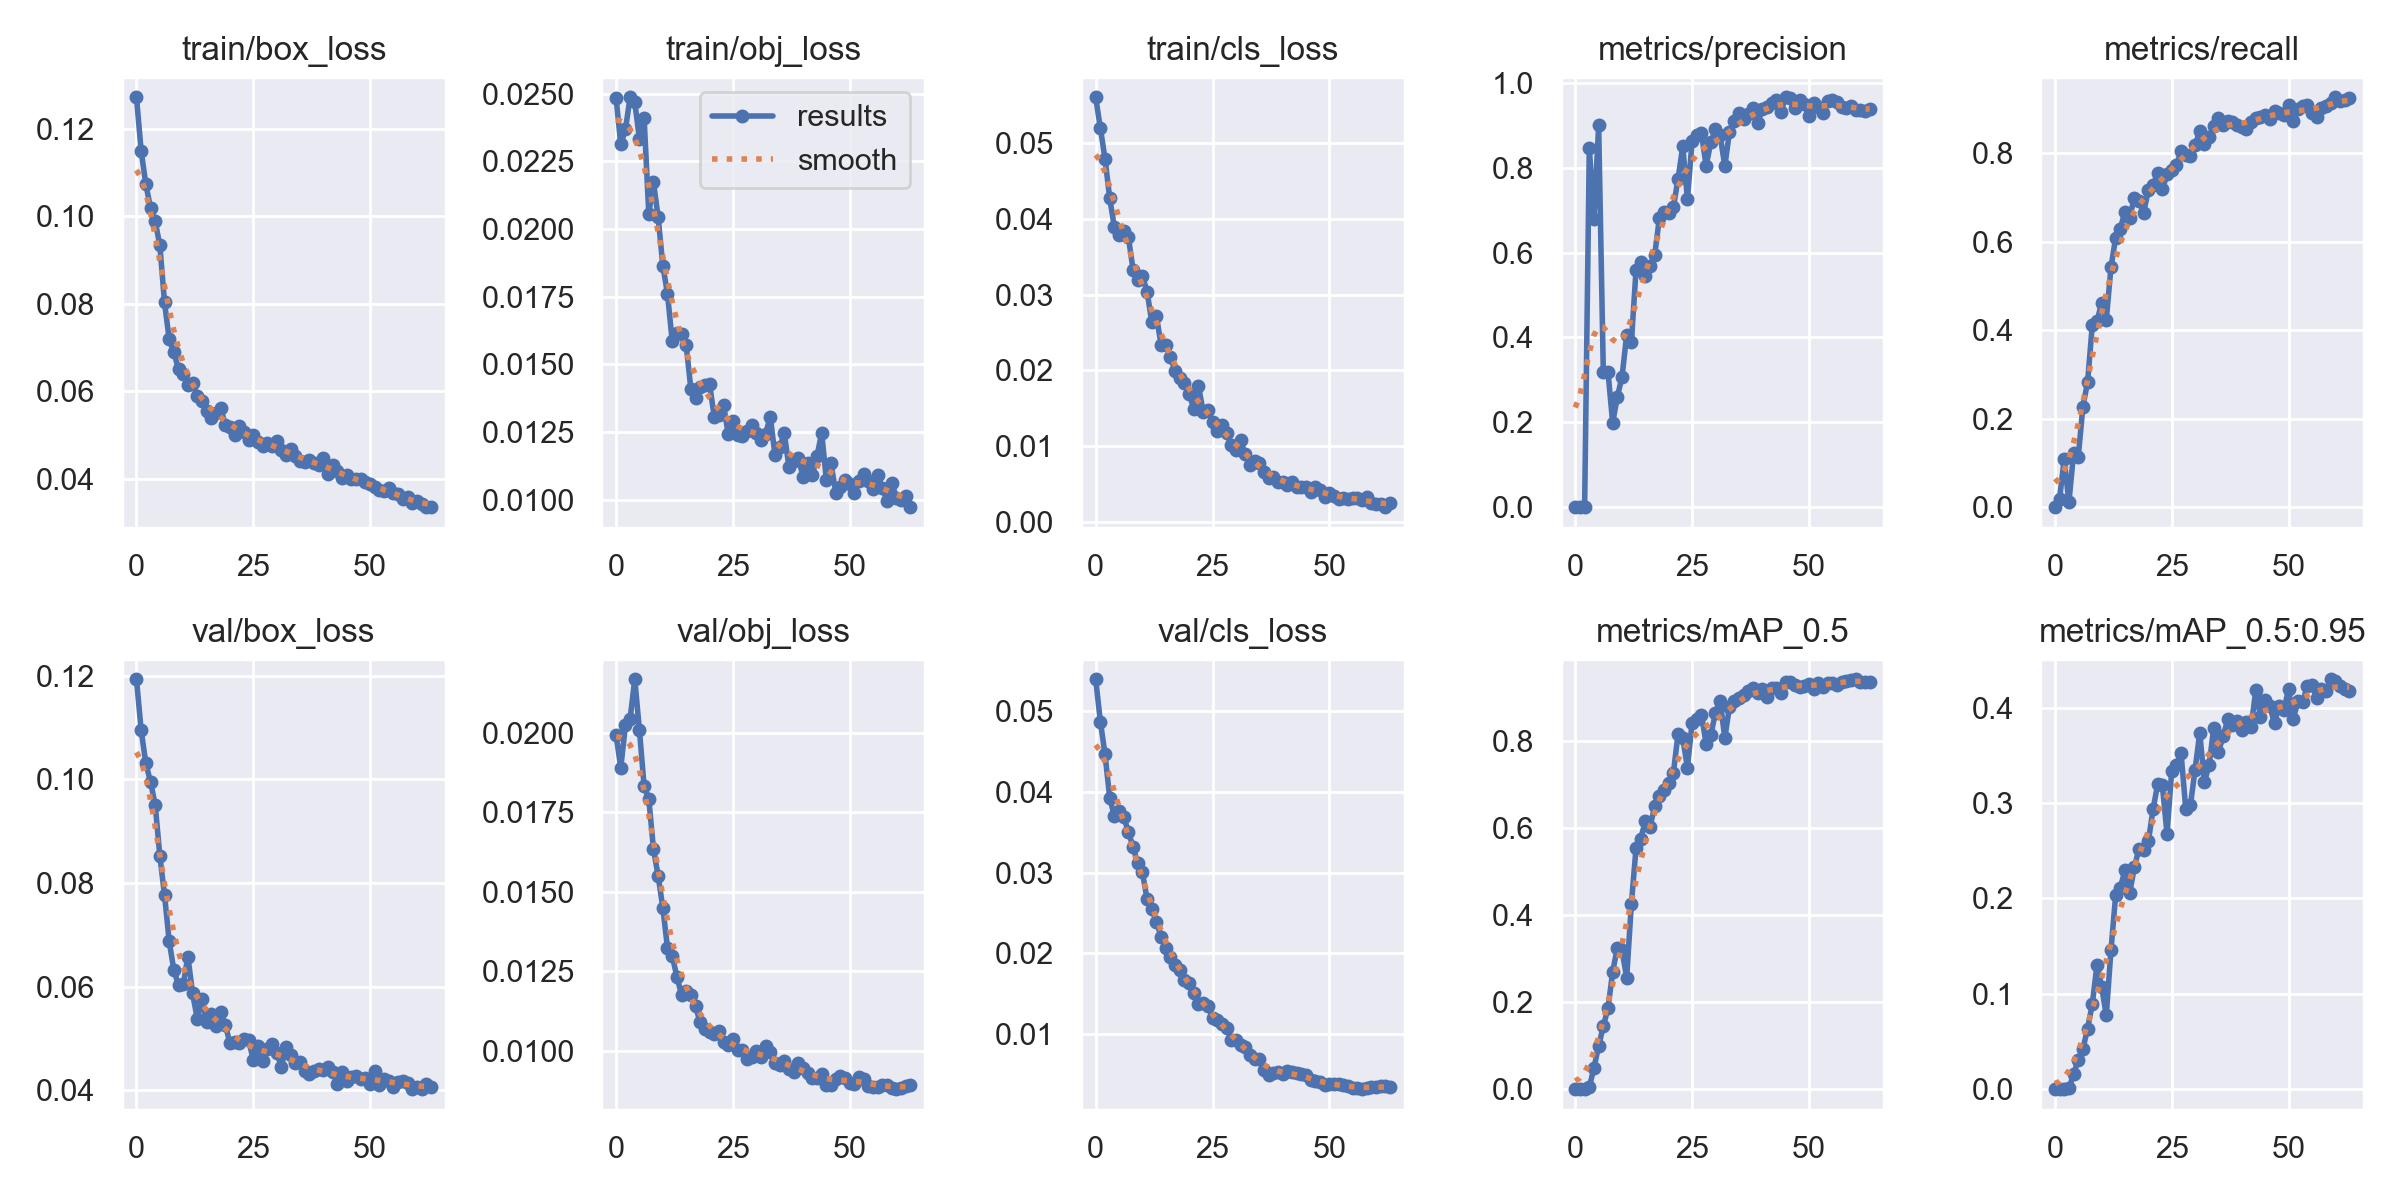
\includegraphics[width=1\paperwidth,height=1\paperheight,keepaspectratio]{./graphics/graphs_yolo.png}
    \end{turn}
    \caption{Metrics for Res-Unet model}
    \label{fig:graphs_yolo}
\end{figure}
\restoregeometry

\clearpage
%\newpage

Confusion matrix : (See Fig.~\ref{fig:confusion_yolo}.).
\begin{figure}[H]
    \centering
    \begin{turn}{270}
    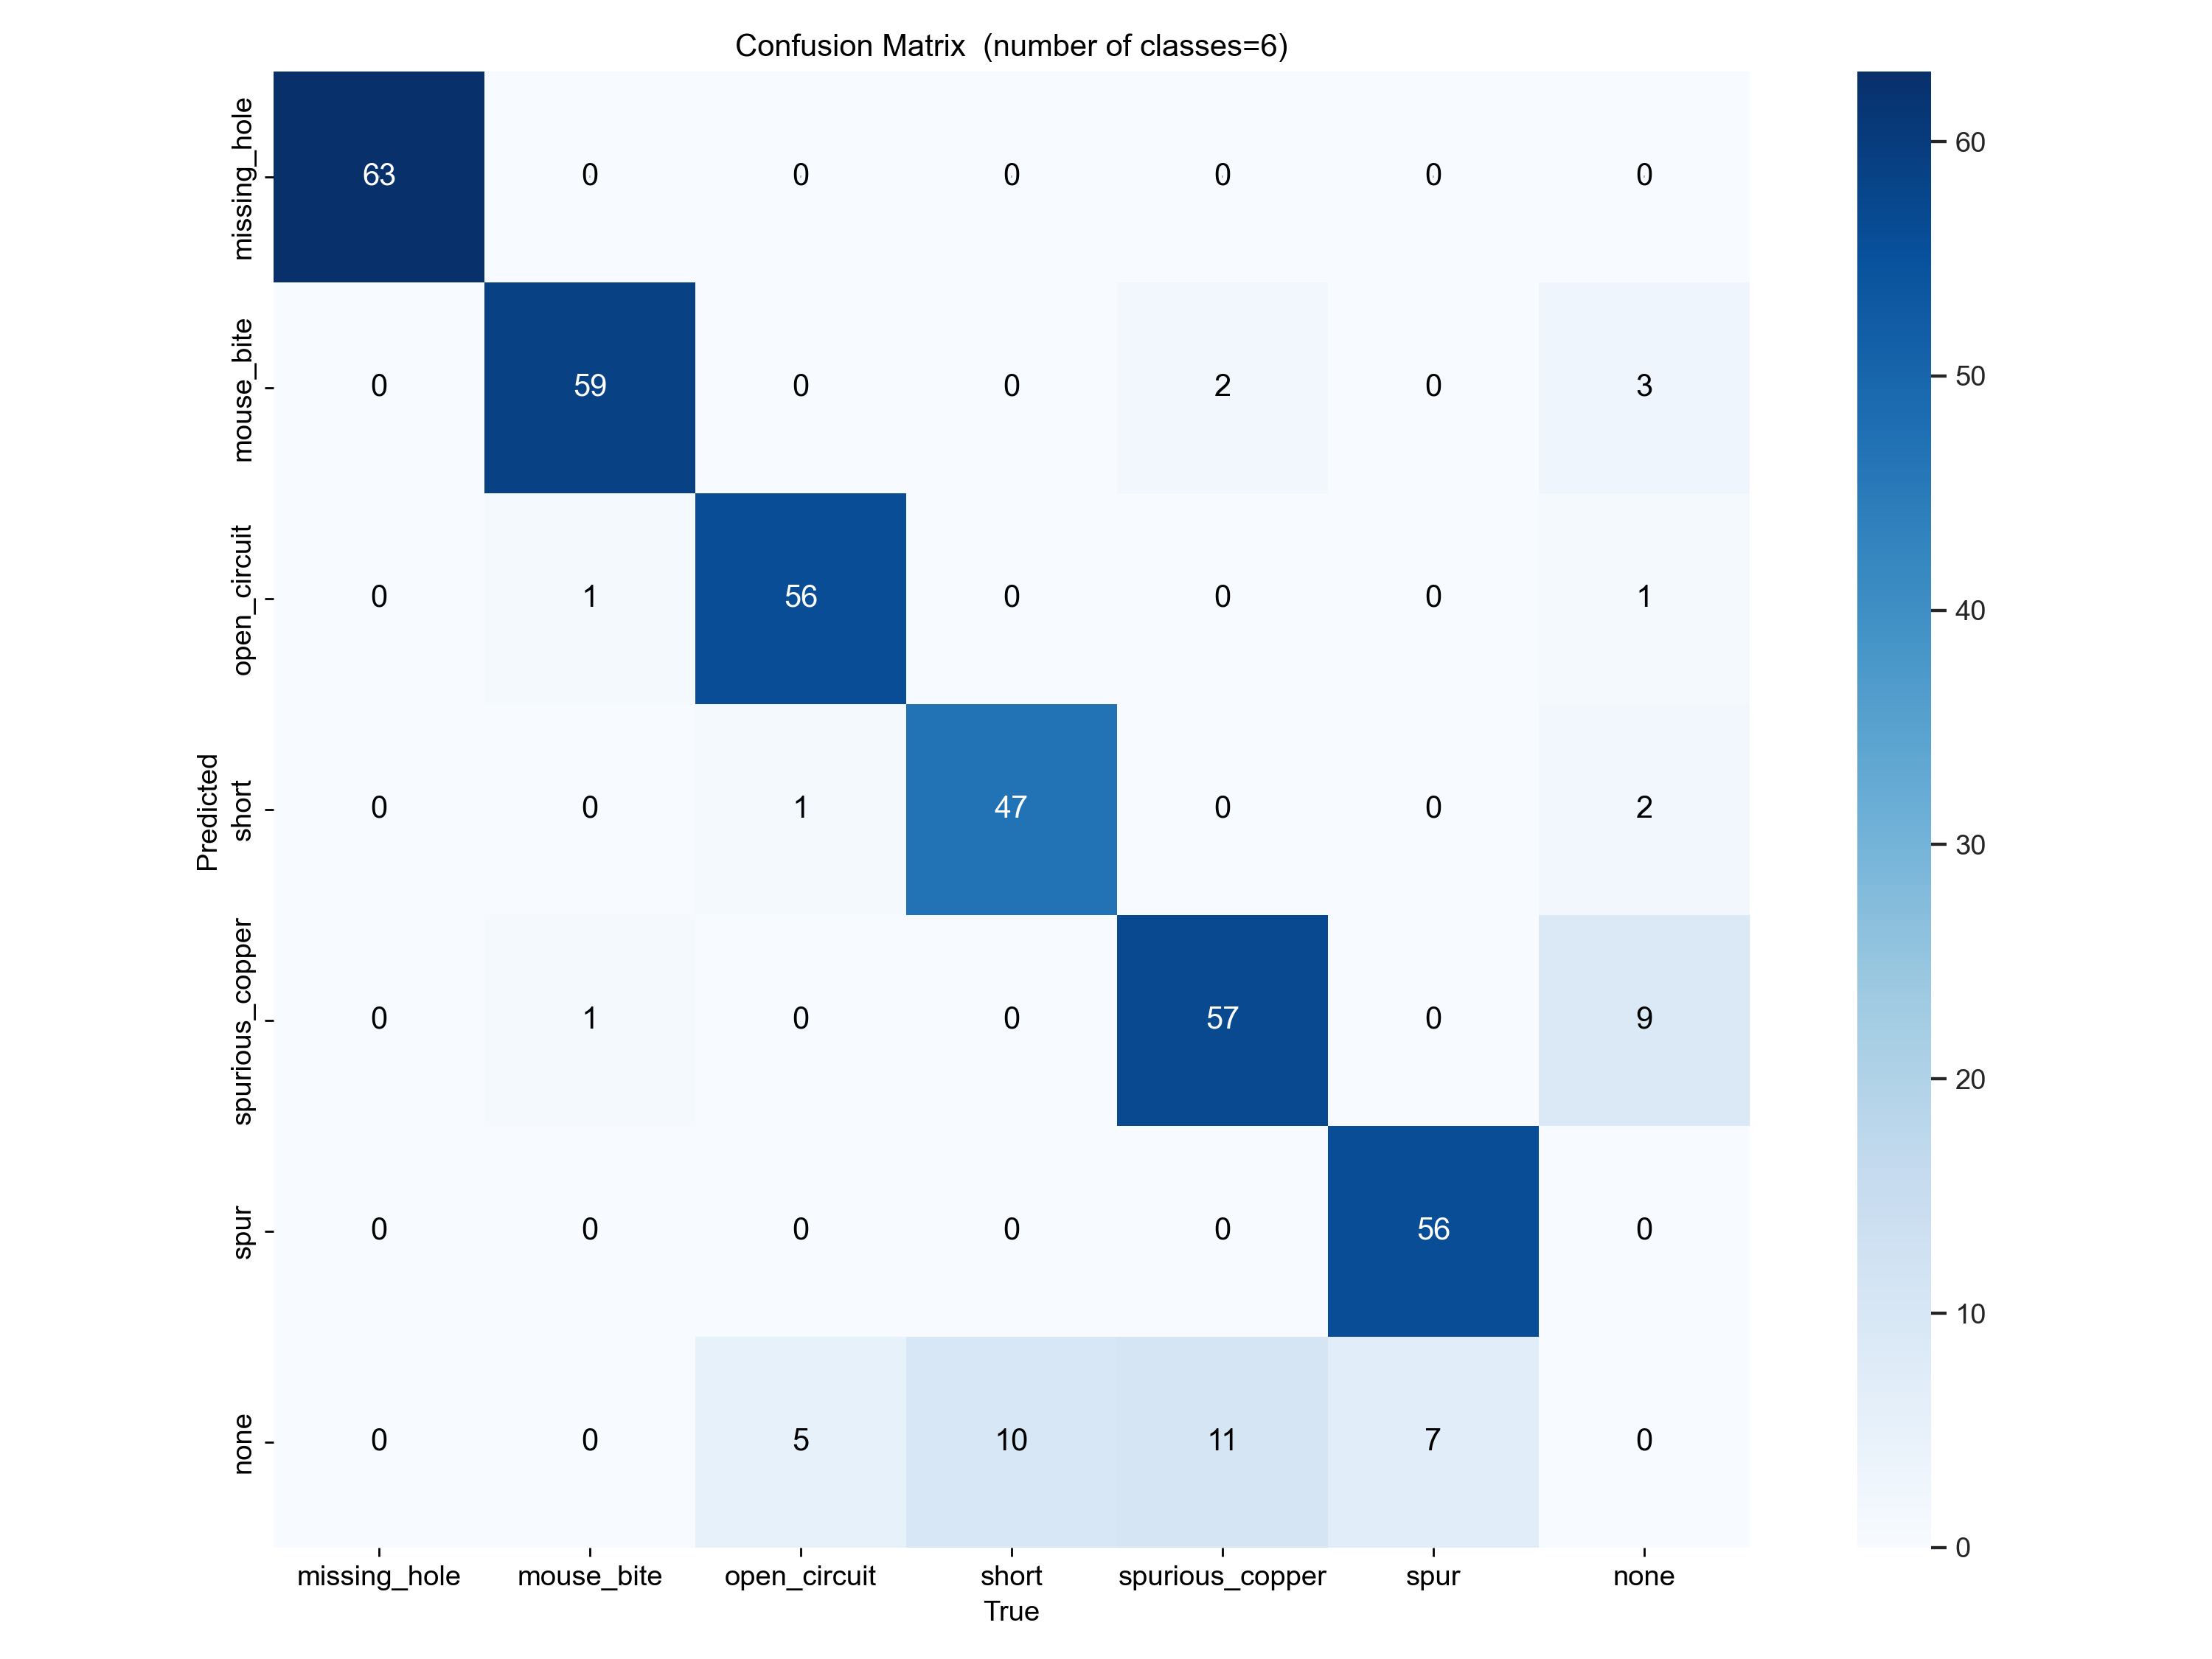
\includegraphics[width=0.7\paperwidth,height=0.7\paperheight,keepaspectratio]{./graphics/confusion_matrix_yolo.png}
    \end{turn}
    \caption{Confusion Matrix for classification output}
    \label{fig:confusion_yolo}
\end{figure}

\clearpage

\begin{figure}[H]
    \centering
    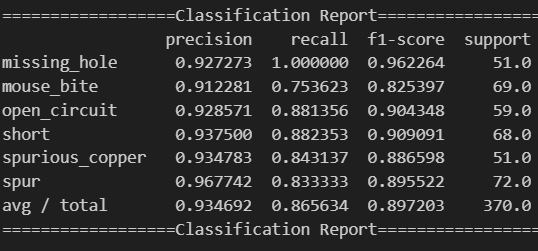
\includegraphics[width=1\textwidth]{./graphics/classification_report_yolo.png}
    \caption{Classification metrics for classification output}
    \label{fig:classification_report_yolo}
\end{figure}

\clearpage

\subsubsection{YOLOv5 model Results}
The results for prediction on validation data can be seen in the following figures. The results are very accurate, but there are still undetected defects e.g. in Fig.~\ref{fig:results1_yolo}, the open circuit image has 2 defects whereas only one was detected.
\begin{figure}[h]
    \centering
    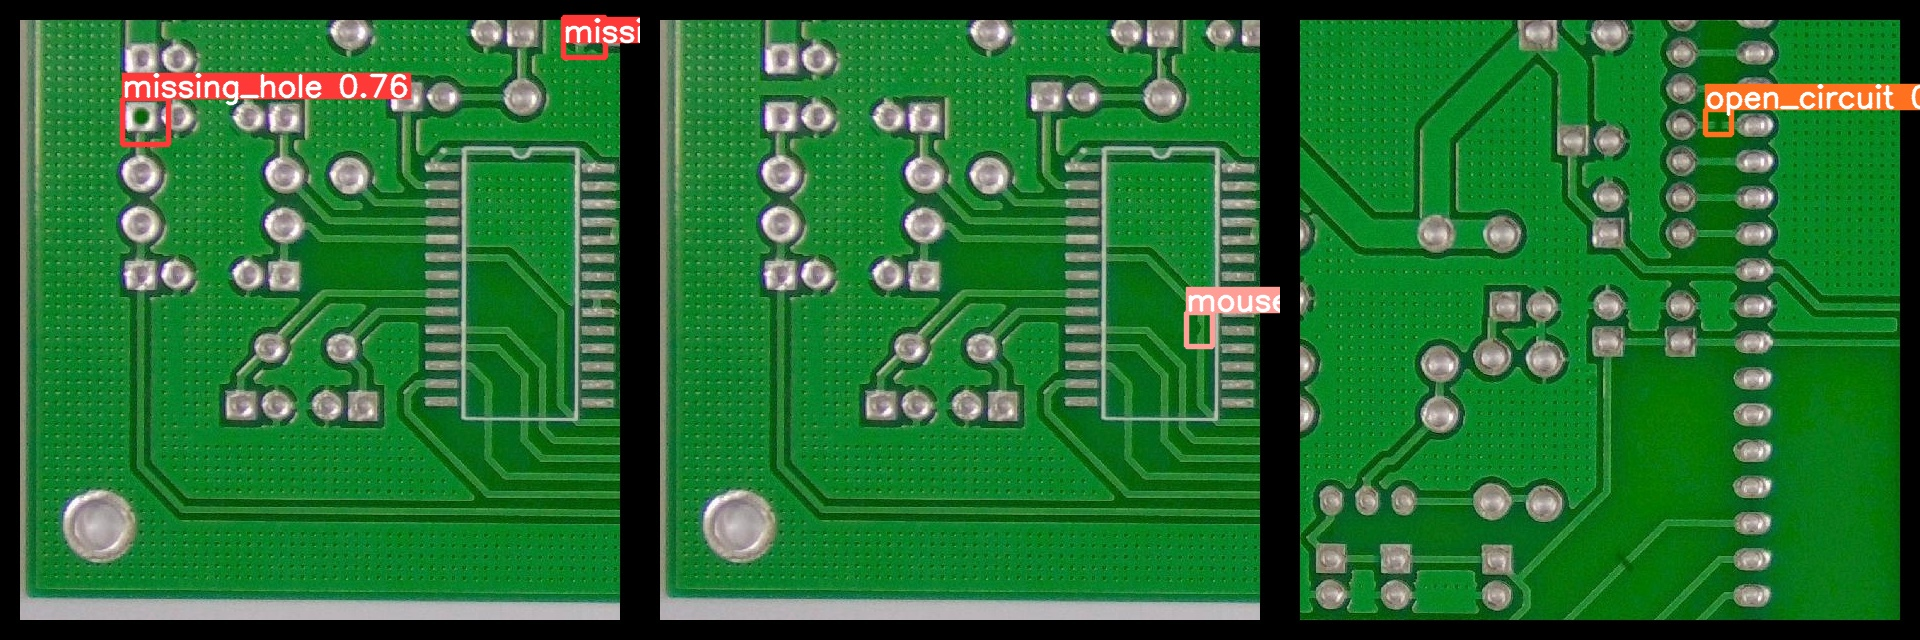
\includegraphics[width=0.8\textwidth]{./graphics/results1_yolo.png}
    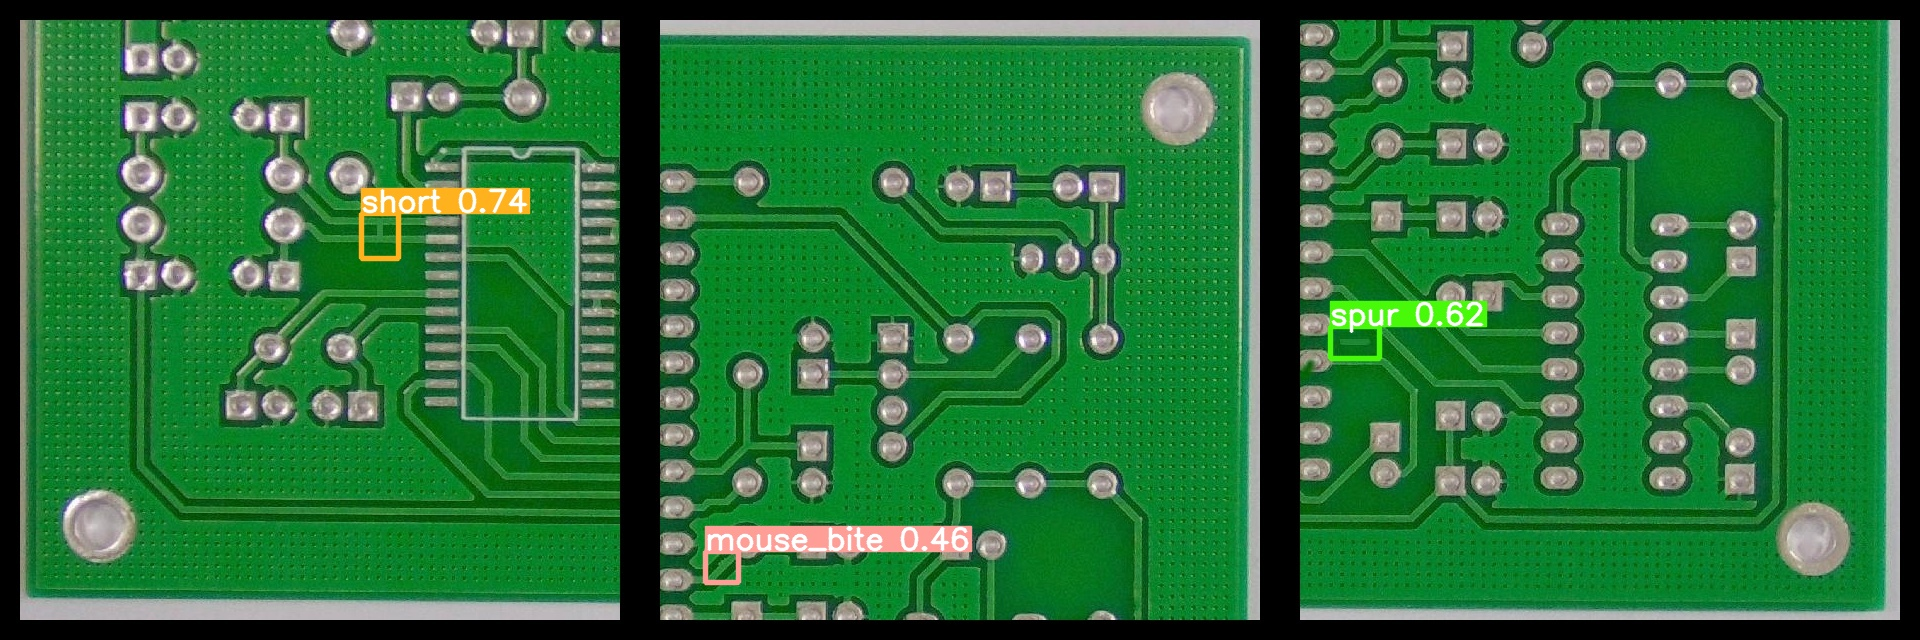
\includegraphics[width=0.8\textwidth]{./graphics/results2_yolo.png}
    \caption{Validation Results}
    \label{fig:results1_yolo}
\end{figure}
\begin{figure}[h]
    \centering
    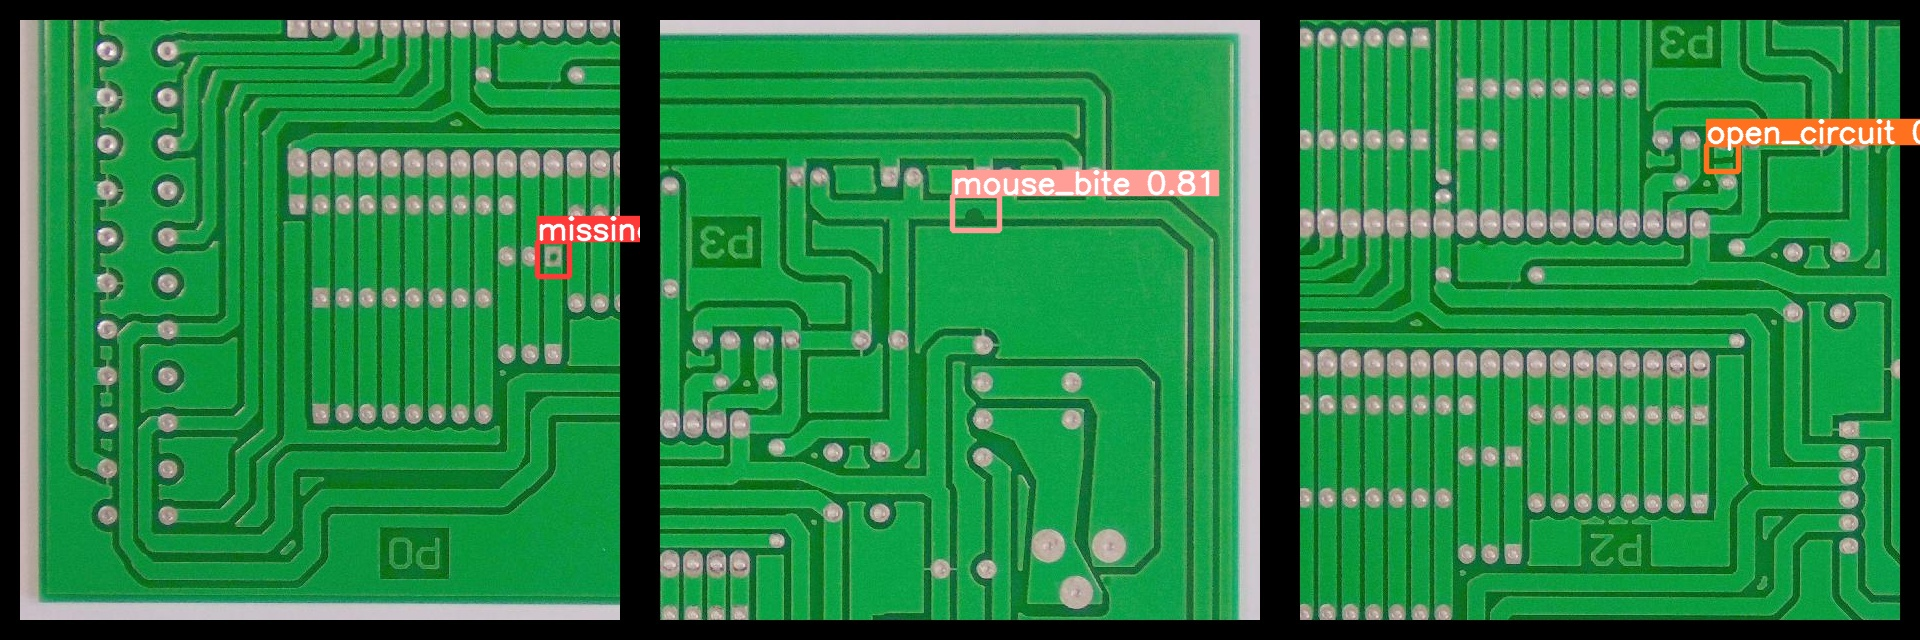
\includegraphics[width=0.8\textwidth]{./graphics/results3_yolo.png}
    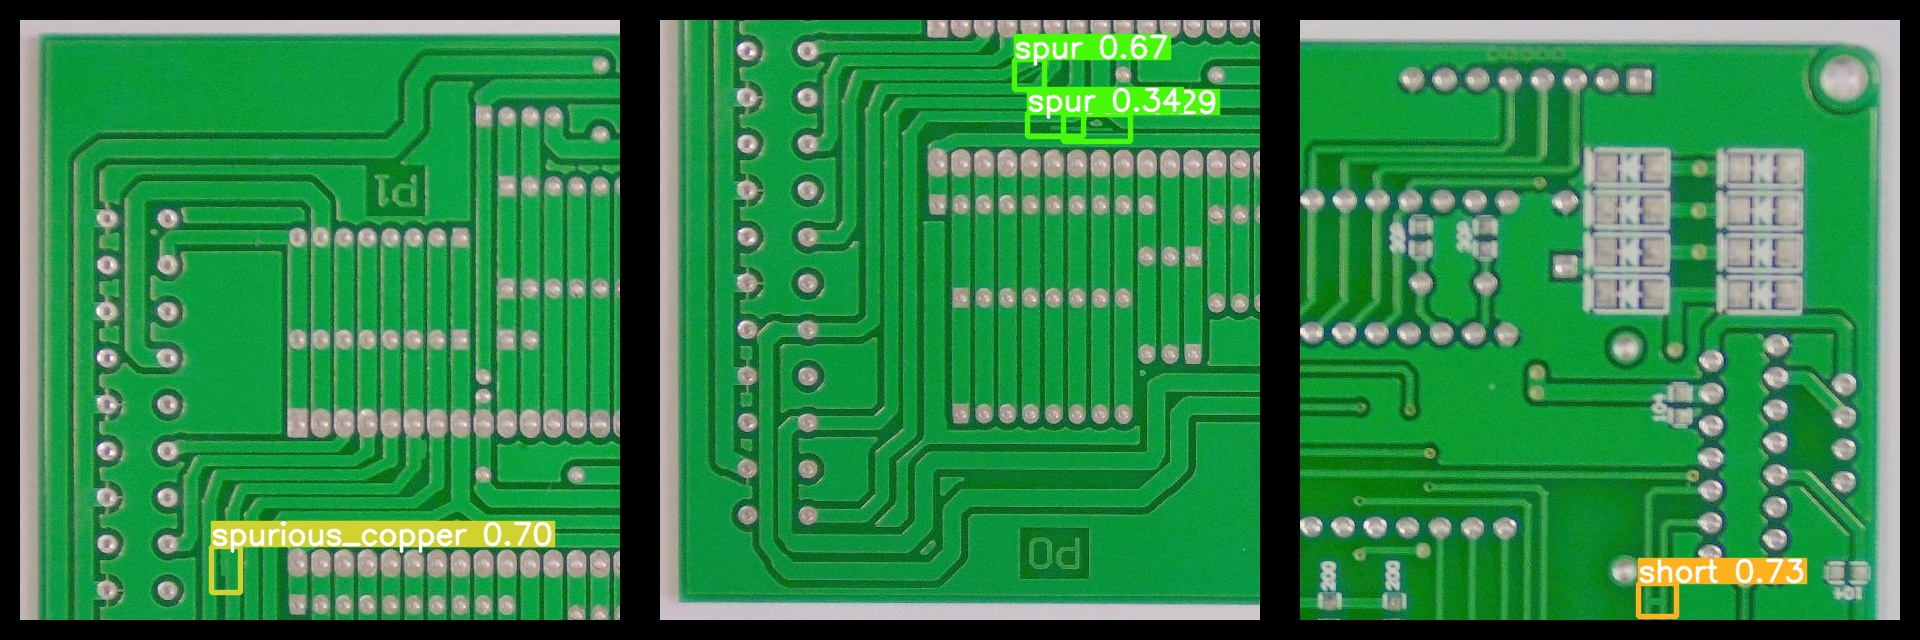
\includegraphics[width=0.8\textwidth]{./graphics/results4_yolo.png}
    \caption{Validation Results}
    \label{fig:results2_yolo}
\end{figure}

\clearpage
\newpage

\subsection{Model Interpretability}
Model interpretability is crucial for understanding the decisions made by deep learning models, especially in complex tasks like image segmentation and classification. 
Since our project was a comprehensive image detection project(segmentation and classification); we had to implement an approach for understanding the behavior and decision-making process of the deep learning model. Implementing such behavioural interpretation can help understand the strengths and weaknesses of the model and guide us in improving its trustworthiness and reliability.

\subsubsection{Grad-Cam}

\begin{figure}[h]
    \centering
    \begin{subfigure}[b]{0.45\textwidth}
        \centering
        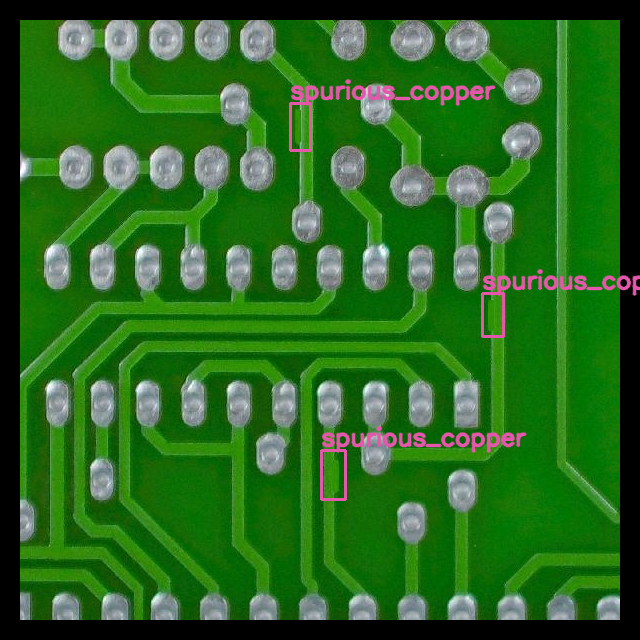
\includegraphics[width=\textwidth]{./graphics/testing_gradcam_yolo.png}
        \caption{Original image}
        \label{fig:image1}
    \end{subfigure}
    \hfill
    \begin{subfigure}[b]{0.45\textwidth}
        \centering
        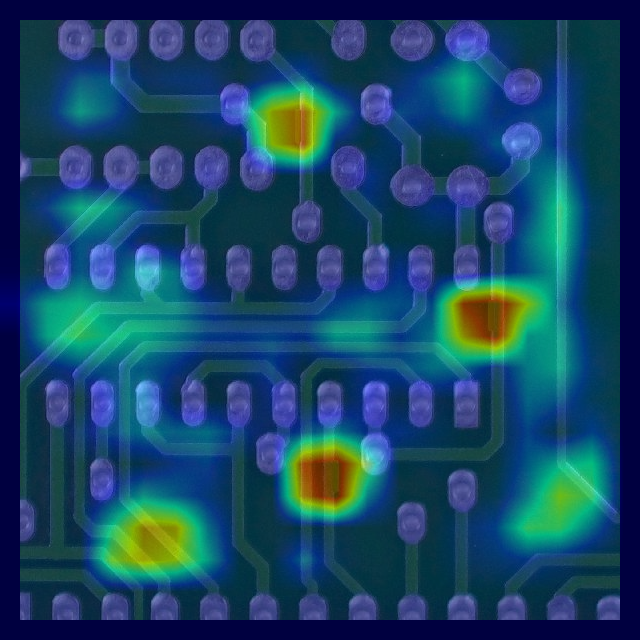
\includegraphics[width=\textwidth]{./graphics/gradcam_yolo.png}
        \caption{Grad-Cam Segmentation Result}
        \label{fig:image2}
    \end{subfigure}
    \caption{Grad-Cam results for YOLOv5}
    \label{fig:gradcam_yolo}
\end{figure}

We implemented Grad-Cam for the YOLOv5 model. Keeping in mind that this is not a comprehensive study on the model's interpretability and therefore does not reflect the results obtained for prediction accurately, the results obtained provide a good outlook for the model behaviour. 
Model interpretability is a massive field of study that can be further explored in the future for a comprehensive understanding of the model behavior.

\clearpage
\newpage

\section{Conclusion}

The machine learning approach for defect detection and classification on PCBs demonstrates significant potential for improving the quality control process in PCB manufacturing. 

\subsection{RES-UNET architecture}
While the classic U-NET architecture was sufficient to achieve already high metric values in the segmentation, it was not before we combined it with residual blocks in each encoding and decoding step of the UNET (RES-UNET) that the accuracy of the classification branch moved to acceptable levels. In fact, the RES-UNET model demonstrated high accuracy in detecting and classifying PCB defects, proving to be a robust solution for PCB defect detection. The combined architecture of Residual Networks and UNET provided the necessary features for precise defect segmentation and classification,  with a segmentation and classification accuracy of about ~97\% and ~90\%, respectively, on our chosen dataset. This evaluation highlights the successful application of the RES-UNET model, providing a strong foundation for further enhancements and deployment in real-world PCB inspection scenarios.

Hence we can conclude that the model works very well on our chosen dataset.

\subsection{YOLOv5 architecture}
The YOLOv5 model, with its high accuracy and efficiency, shows promise for real-time defect detection. Future work will focus on enhancing the models' performance by incorporating fine tuning training weights, improving data augmentation techniques, and exploring other advanced interpretability techniques.

\clearpage
\newpage

\section{Future Work}
We observed many areas of improvement for future scope of work. 
\begin{itemize}
    \item The training metrics indicate that additional epochs could yield better results. Due to computational and time constraints, we limited each model to 50 epochs. A key improvement would be to train or retrain the models for 100 epochs.
    \item There is potential in leveraging a computationally powerful computer with a GPU for machine learning which can significantly enhance data processing. Currently, extensive pre-processing is required to prepare the small-scale images for training.
    \item It is crucial that DataScientest provide students with remote virtual machines equipped with GPU's so that the model training could be done with more efficiency.
    \item More metrics can be observed for the current architecture including Dice Coefficient, Precision-Recall Curve, etc.  
    \item For training the Res-UNet model, the augmented training and testing datasets were initially loaded into memory as arrays, consuming a considerable amount of RAM. To optimize RAM utilization, an alternative approach involved saving the images to the hard disk and subsequently loading them in batches during training. This strategy effectively mitigated RAM usage, thereby enabling the model to make more efficient use of available memory resources.
    \item Class of defects were limited for this project. Including wafer cracks, copper detachment, component misalignment or damage, etc for future learning will improve model performance in scenarios with real-life defects.
    \item The image dataset used in this project is very academical in the sense that the PCBs are plain and have no further components attached to them. In a real world application one is interested in defects on the board especially after the attachment of further components to the PCB. This would greatly increase the variety of possible input imagery including shapes and contours our model has not been trained on. Train the model on real world images from PCBs during or at the end of the production process will enable the model to be used in more practical scenarios.

\end{itemize}
\clearpage
\newpage

\begin{thebibliography}{10} 
    \bibitem{Ixiaohuihuihui}
    Ixiaohuihuihui. (2021). Tiny Defect Detection for PCB. GitHub Repository. Available online: \\\url{https://github.com/Ixiaohuihuihui/Tiny-Defect-Detection-for-PCB}.
    
    \bibitem{Wang2022}
    Wang, X., Yang, F., Zhang, X. (2022). A novel self-supervised adversarial learning method for defect detection on printed circuit boards. \textit{Journal of Manufacturing Systems}, \textbf{63}, 340-352. DOI: \url{https://doi.org/10.1016/j.jmsy.2021.09.006}.
    
    \bibitem{Akhatova2021}
    Akhatova, A. (2021). PCB Defects. Kaggle Dataset. Available online: \url{https://www.kaggle.com/datasets/akhatova/pcb-defects/data}.
    
    \bibitem{Brownlee2022}
    Brownlee, J. (2022). How to Perform Object Detection With YOLOv3 in Keras. Machine Learning Mastery. Available online: \url{https://machinelearningmastery.com/how-to-perform-object-detection-with-yolov3-in-keras/}.
    
    \bibitem{Zhao2020}
    Zhao, H., Lin, Z., Fu, Y., et al. (2020). Residual-Attention UNet++: A Nested Residual-Attention U-Net for Medical Image Segmentation. \textit{IEEE Transactions on Neural Networks and Learning Systems}, \textbf{32}(4), 1539-1553. DOI: \url{https://doi.org/10.1109/TNNLS.2020.3011597}.

    \bibitem{Kim2021}
    Kim, M., Jeong, J., Kim, S. (2021). ECAP-YOLO: Efficient Channel Attention Pyramid YOLO for Small Object Detection in Aerial Image. \textit{Remote Sensing}, \textbf{13}(11), 4851. DOI: \url{https://doi.org/10.3390/rs13234851}.

    \bibitem{Gildenblat2024}
    Jacob Gildenblat, "Advanced AI Explainability with PyTorch-GradCAM," 2024. [Online]. Available: \url{https://jacobgil.github.io/pytorch-gradcam-book/}.

    \bibitem{TensorFlowAPI}
    TensorFlow. (n.d.). \textit{tf.keras.losses}. Retrieved June 17, 2024, from \url{https://www.tensorflow.org/api_docs/python/tf/keras/losses}


    
\end{thebibliography}

\clearpage
\newpage

\end{document}
